\documentclass[11pt]{article}
\usepackage{coling2016}
\usepackage{times}
\usepackage{url}
\usepackage{wrapfig}
\usepackage{graphicx}
\graphicspath{ {images/} }
%\bibliographystyle{acl}
%\bibliography{coling2016}

\title{Learning to Solve Arithmetic Word Problems using Sentence Simplification}

\author{First Author \\
  Affiliation / Address line 1 \\
  Affiliation / Address line 2 \\
  Affiliation / Address line 3 \\
  {\tt email@domain} \\\And
  Second Author \\
  Affiliation / Address line 1 \\
  Affiliation / Address line 2 \\
  Affiliation / Address line 3 \\
  {\tt email@domain} \\}
  
\begin{document}
\maketitle
\begin{abstract}
  This paper presents a sentence simplification approach to learning to solve arithmetic word problems. The approach performs a thorough analysis of each sentence in the given word problem to map each sentence to a simplified syntactic pattern. The syntactic pattern is generated by parsing the sentence using a dependency parser and encapsulates all the relevant information in a sentence including the subject, verb and object with its quantity as shown in Figure 1. The pattern is then used as a feature alongside other features as described in the Features section to classify the operator of the object given in the sentence. The classifier is trained on a small dataset of sentences and their operators and is not manually annotated. An equation is generated using similar information from multiple sentences in a given word problem.

  Using this approach the system learns to classify the operator with 70\% and is able to solve 70\% of the problems in the public dataset released by ~\cite{Hosseini:14} and can be found online\footnote{Dataset used is available at \url{https://www.cs.washington.edu/nlp/arithmetic}.}. The system overcomes some of the parsing issues encountered in attempt to solve word problems before and needs some improvement around the relational errors.
\end{abstract}
 
\section{Introduction}
\label{Intro}
Mathematical word problems are generally a sequence of actions by a subject on an object. The challenge in solving mathematical word problems is to extract information from a sentence accurately. Converting the extracted information to an equation is a trivial part. The complexities in extracting information increases when the sentence refers to an entity encountered in the previous sentences or some other related entities such as dollars and money.\newline

\begin{figure}[h]
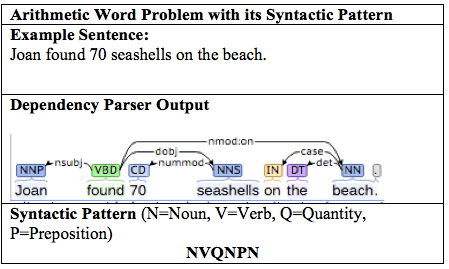
\includegraphics[width=0.6\textwidth]{Figure1}
\centering
\caption{\label{fig:Figure1}Example sentence of a word problem and its syntactic pattern.}
\end{figure}

When taking word problems into consideration, Algebra may be a challenging part from a child's point of view but the semantics of a sentence such as understanding of the syntax, extensive knowledge, coreference resolution and extracting information from individual sentences and combine that information effectively to produce a result.\newline

Our system needs to parse the sentences in a word problem well to fetch useful information. This information needs to be used collectively in an effective way to generate an equation. Solving the equation if generated correctly is a trivial part. Figure 1 shows an example of how a sentence from a word problem is simplified to a syntactic pattern. This paper approaches the problem of solving arithmetic word problems by mapping individual sentences in a word problem to a syntactic pattern. Based on the syntactic pattern each sentence is simplified till it represents minified information which consists of a subject, verb, object with its quantity and preposition if there exists one. This simplified sentence is then classified to an operator and the object with its quantity is added to the equation with the classified operator. Each simplified sentence is classified to one of four operators as described in Table ?.\newline 

We gather information form the sentences by parsing the sentence using the dependency parser \footnote{http://nlp.stanford.edu/software/stanford-dependencies.shtml}. Based on the Part-of-speech tags and relations between the words from the sentence different entities from the sentence are extracted. Expletives, nouns and their quantities, verbs,  conjunctions, adjectives and prepositions are extracted from the sentence and are related to each other based on the relations output by the dependency parser. Based on some rules these extracted entities are used collectively to form a simplified sentence and is provided as an input to the classifier. As explained above the classifier predicts an operator for the simplified sentence. Now that we have the operator we use the operator and the extracted entity in the equation. Consider the below example:
\begin{figure}[h]
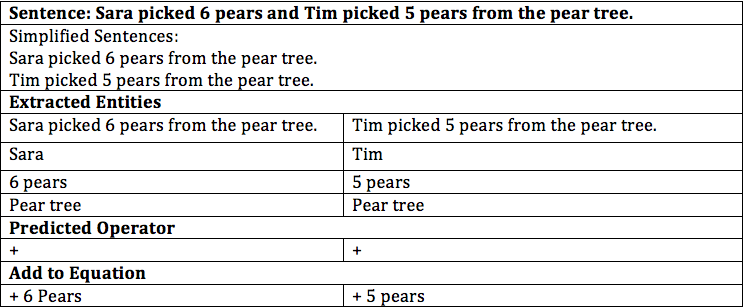
\includegraphics[width=0.90\textwidth]{Figure2}
\centering
\caption{\label{fig:Figure2}Example sentence of a word problem and its simplification.}
\end{figure}

Simplifying the sentences to such format makes this less complex for the classifier as well as to generate equations. Though the training data seems to be the sentences, actually the sentences are just a way to generate syntactic patterns which are used extensively as the features to the classifier. A large number of sentences will end up having the same syntactic pattern. Hence, training is actually on syntactic patterns and not on raw text. Our system is evaluated on an existing dataset of arithmetic problems provided by ~\cite{Hosseini:14}. \newline

Our system learns this classifier based on 300 individual sentences. Our data and source code are publicly available \footnote{Source code and training dataset is available at \url{https://github.com/vishalrajpal/TrySystem}.}. The next section describes how we extract the syntactic pattern, its usage and problem decomposition.


\section{Syntactic Pattern and Problem Decomposition}
\label{method}
In this section we describe how we use the dependency parser output to extract the syntactic pattern of a sentence and the process of simplifying sentences using the extracted syntactic pattern. We further describe the way we predict the operator of the simplified sentence using a Logistic Regression classifier. The input to our system is a problem text and we carry out multiple steps for each sentence in this problem text. Below are the steps:

\subsection{Run Dependency Parser on Each Sentence}
For each sentence in the problem text, we extract the relations and the part-of-speech tags using the dependency parser. Based on the output from the dependency parser we extract the Expletive if any, Nouns and their quantities, preposition, conjunction etc. and build a syntactic pattern based on the ordering of the words in the sentence as described in Figure 1. The representation of a sentence as a syntactic pattern helps us fetch information about this sentence easily such as if the sentence has a quantified noun or a conjunction, an expletive or a preposition etc. We use this information to further simplify the sentence as described in further steps. 

\subsection{Parse Commas in Each Sentence}
In most arithmetic word problems, commas are a way to either multiple subjects interacting with the same object or a subject interacting with multiple objects. Hence, to simplify sentences comma is an important punctuation character. After extracting the syntactic pattern of the overall sentence, the sentence is looked for commas. If any of the commas exist based on some rules we decide if the text before comma belongs to the subject part of the sentence or the object part of the sentence. The goal of this step is to have simplified sentences based on parsing commas in the sentence. The current sentence is replaced by simplified sentences extracted by parsing the sentence based on a comma. Consider the below example:

\begin{figure}[h]
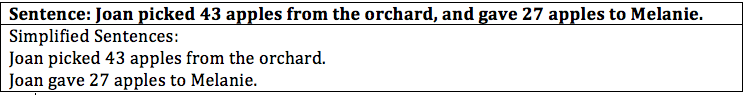
\includegraphics[width=0.90\textwidth]{Figure3}
\centering
\caption{\label{fig:Figure3}Simplification of a sentence based on a comma.}
\end{figure}

\subsection{Run Dependency Parser on Each Sentence}
Now that we have simplified sentences extracted by parsing the sentence based on a comma, we give these simplified sentences to the dependency parser to update the syntactic pattern. The syntactic pattern is extracted in the same way as in Step 2.1. We further apply some rules to extract more simpler sentences.

\subsection{Parse Conjunctions in Each Sentence}
Similar to commas, in most arithmetic problems conjunctions are a way mostly to specify two subjects interacting with a single object, or a single subject interacting with two objects. Based on the updated syntactic pattern from previous step looking if a conjunction exists is trivial. If a conjunction exists we simplify the sentence based on some rules. The goal of this step is to have multiple simplified sentences based on parsing by conjunctions. The current sentence is replaced by simplified sentences extracted by parsing the sentence based on a conjunction. Below is an example where a conjunction "and" exists:

\begin{figure}[h!]
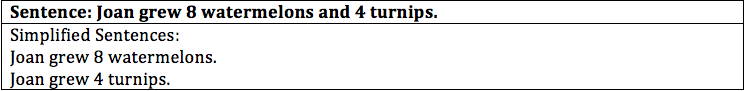
\includegraphics[width=0.90\textwidth]{Figure4}
\centering
\caption{\label{fig:Figure4}Simplification of a sentence based on a conjunction.}
\end{figure}

\subsection{Run Dependency Parser on Each Sentence}
At this point, the sentences are simplified at the most granular level. Since, each sentence is replaced by multiple simplified sentences their will be multiple syntactic patterns. We provide these simplified sentences to the dependency parser and based on the same rules used in the above steps we extract the useful information such as Nouns, verbs etc. Based on the information extracted the features for each sentences are extracted from the syntactic pattern and other properties as described in ?. At this point, we have a feature vector for a single sentence of the problem text. Each sentence of the problem text will be simplified to multiple sentences and each simplified sentence would have its own feature vector which would classified to an operator as discussed in the next step.

\subsection{Features} 
\subsubsection{Syntactic Patterns}
All the syntactic patterns extracted from the training data are used as individual features. The syntactic pattern to which the sentence belongs is et and all the other are not in a one-hot encoding way. From the training data of 300 sentences, we extracted near to 125 syntactic patterns, which shows that multiple sentences have a similar syntactic pattern. For text data, even if we haven't seen a pattern before the other features as described below will try to map the syntactic pattern found to the existing syntactic pattern. 

\subsubsection{Count based Features}
Based on our analysis we found that having a count of some important things in the syntactic pattern proves to be helpful in to the classifier in learning accurately. There are 4 count based features: number of nouns, number of prepositions, number of verbs and number of quantities. These features depend on how we map the sentence to a syntactic pattern and as explained above if we map the sentence to the correct syntactic pattern, extracting these kind of features is a trivial task.

\subsubsection{Occurrence based Features}
\paragraph{Relation based Occurrence Features}
We use the occurrence of some dependency relations as features. Particularly nmod:poss relation from the dependency parser if set can determine the subject possessing the object and nmod:of which helps to differentiate between two nouns of same kind.

\paragraph{Pattern based Occurrence Features}
Occurrence of some specific syntactic pattern as a sub pattern of the syntactic pattern of a sentence can also be helpful. We have 2 features: NVQN syntactic pattern and QN syntactic pattern. These two patterns indicate that a sentence of such pattern is mostly suggesting addition or subtraction.

\paragraph{Word based Occurrence Features}
Some specific words allow the classifier to predict more accurately. The word "now" is suggesting a result after some operation and hence the predicted operator should be "=". Similarly, occurrence of one of the words from "most", "some" and "several" suggests an unknown quantity in the sentence. There are different such words through which we can predict the operation and hence we use the occurrence of such words as features.

\subsubsection{Word similarity based features}
We identified 8 word categories from WordNet and Word2Vec which can be helpful in predicting the operator. The 8 verb categories are "verb.possession", "verb.change", "verb.communication", "verb.consumption" , "verb.contact", "verb.creation", "verb.motion" and "verb.weather". The verbs in the sentence are given as input to WordNet and Word2Vec and the result is normalized between these categories.

\subsection{Training the Classifier to Predict Operator}
At this point we only consider addition subtraction problems but based on our approach and analysis we believe it is generalizable to multiplication and division problems. The possible operators in our system currently are "+", "-", "=" and "?". The "+" operator and "-" are self explanatory, whereas a sentence classified as "=" is suggesting that the quantity in the sentence is a result of some operations and a sentence classified as "?" is suggesting that the sentence is asking a question about some entity.

We train four Logistic Regression binary classifiers for each of the above mentioned operators. We then use one vs all technique to combine the results from these binary classifiers. Our test data contain 55 simplified sentences and the accuracy is as follows:

%Should we have precision and recall?%

\subsection{Using Quantified Noun in the Equation}
Based on the information extracted and the operator to which the sentence is classified, an equation is created or modified either by adding quantified nouns to the equation with its operator or an unknown quantity which needs to be calculated. For Example: The equation based on the extracted information for "Joan has 20 dollars. She gave 10 dollars to his friend. How many dollars does she have now?" will be +20 - 10 = ?.

\begin{thebibliography}{}
  
  \bibitem[\protect\citename{Hosseini \bgroup et al.\egroup}2014]{Hosseini:14}
  Mohammad Javed Hosseini, Hannaneh Hajishirzi, Oren Etzioni and Nate Kushman.
  \newblock 2014.
  \newblock {\em In Proceedings of the EMNLP}
  
\end{thebibliography}

\end{document}